\subsubsection{Backend}
ได้มีการจัดเก็บข้อมูลตลาดหุ้น, ตลาด crypto currency และสร้างระบบอัพเดตข้อมูลอัตโนมัติ ได้เขียนโปรแกรมสำหรับ Fuzzy Logic ไปบางส่วนแล้ว
รวมถึงมีการลองทำตัวเว็บเซิร์ฟเวอร์ไปบ้าง โดยสามารถดู code ได้ที่ \url{https://github.com/Fuzzy-Technical-Indicator/backend}

\begin{figure}[ht]
    \centering
    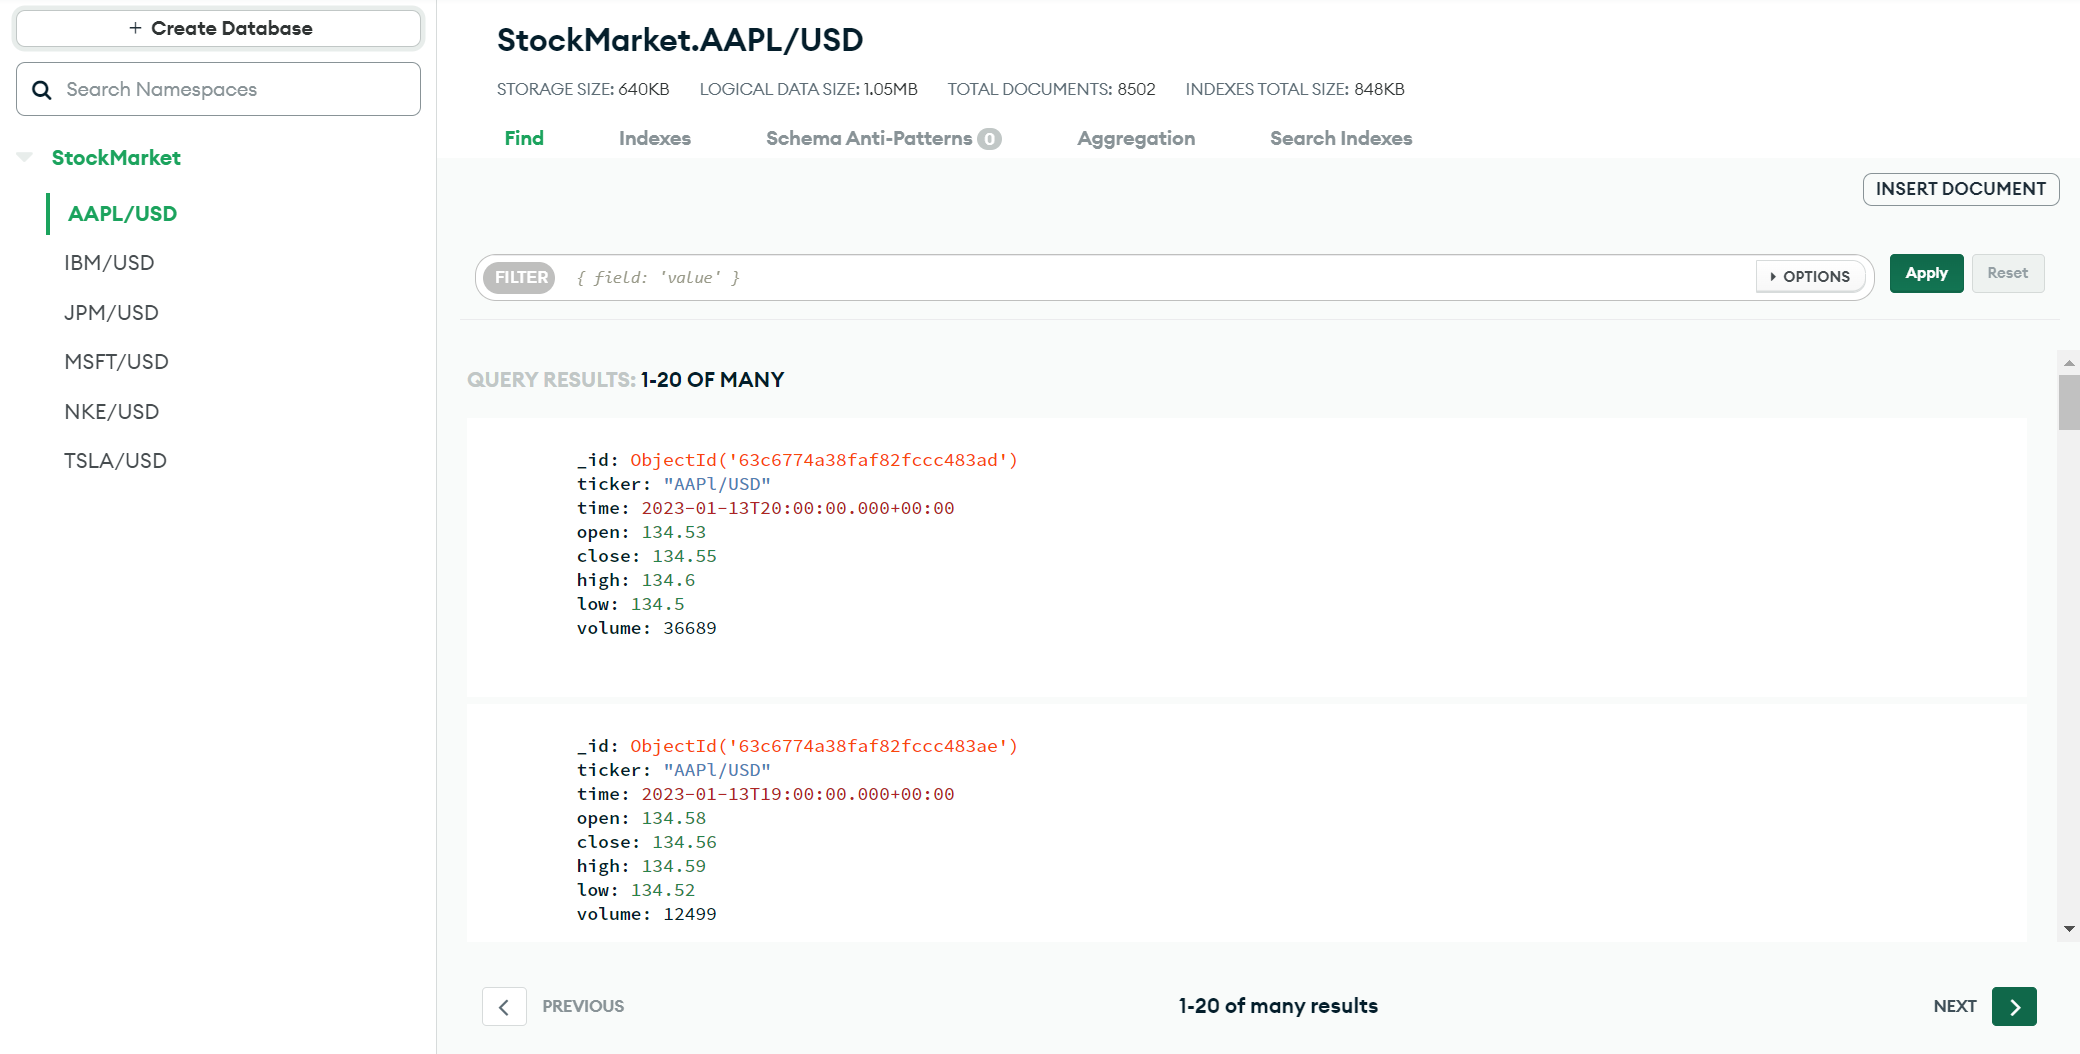
\includegraphics[width=\textwidth]{images/db_example.png}
    \caption{ตัวอย่างข้อมูลตลาดหุ้นในฐานข้อมูล}
\end{figure}
\pagebreak

\subsubsection{Frontend}
ได้มีการออกแบบหน้าตาแอปพลิเคชันทั้งแบบบนเว็บไซต์และแบบโทรศัพท์
\begin{figure}[ht]
    \centering
    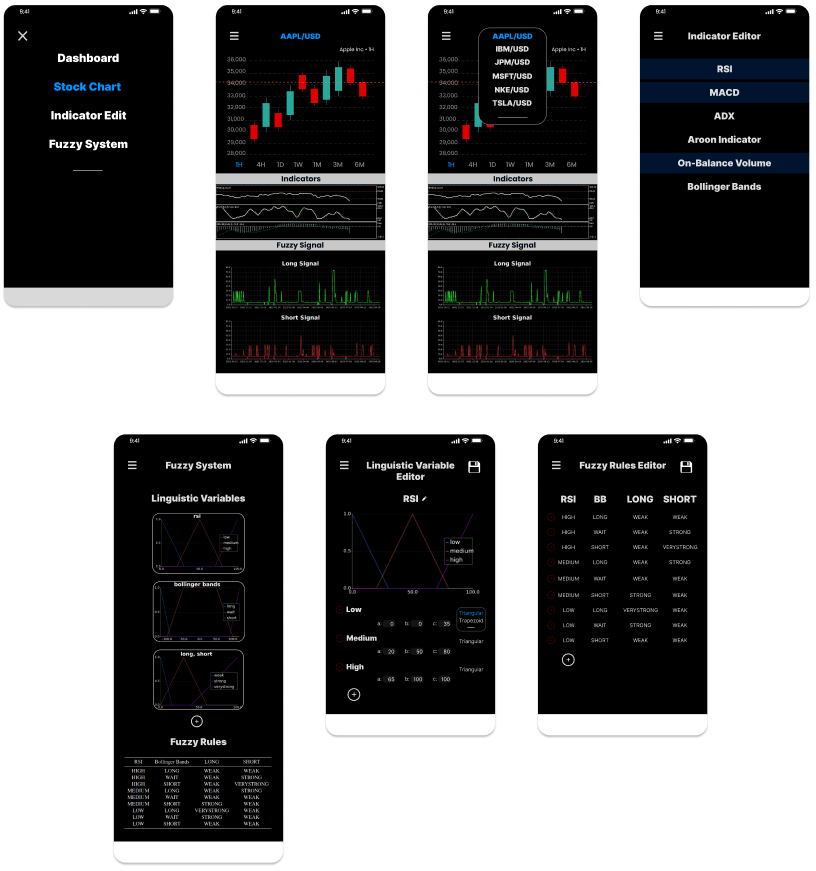
\includegraphics[width=\textwidth]{images/mobile_uiux.png}
    \caption{UI/UX ของแอปพลิเคชันบนโทรศัพท์}
\end{figure}

\begin{figure}[ht]
    \centering
    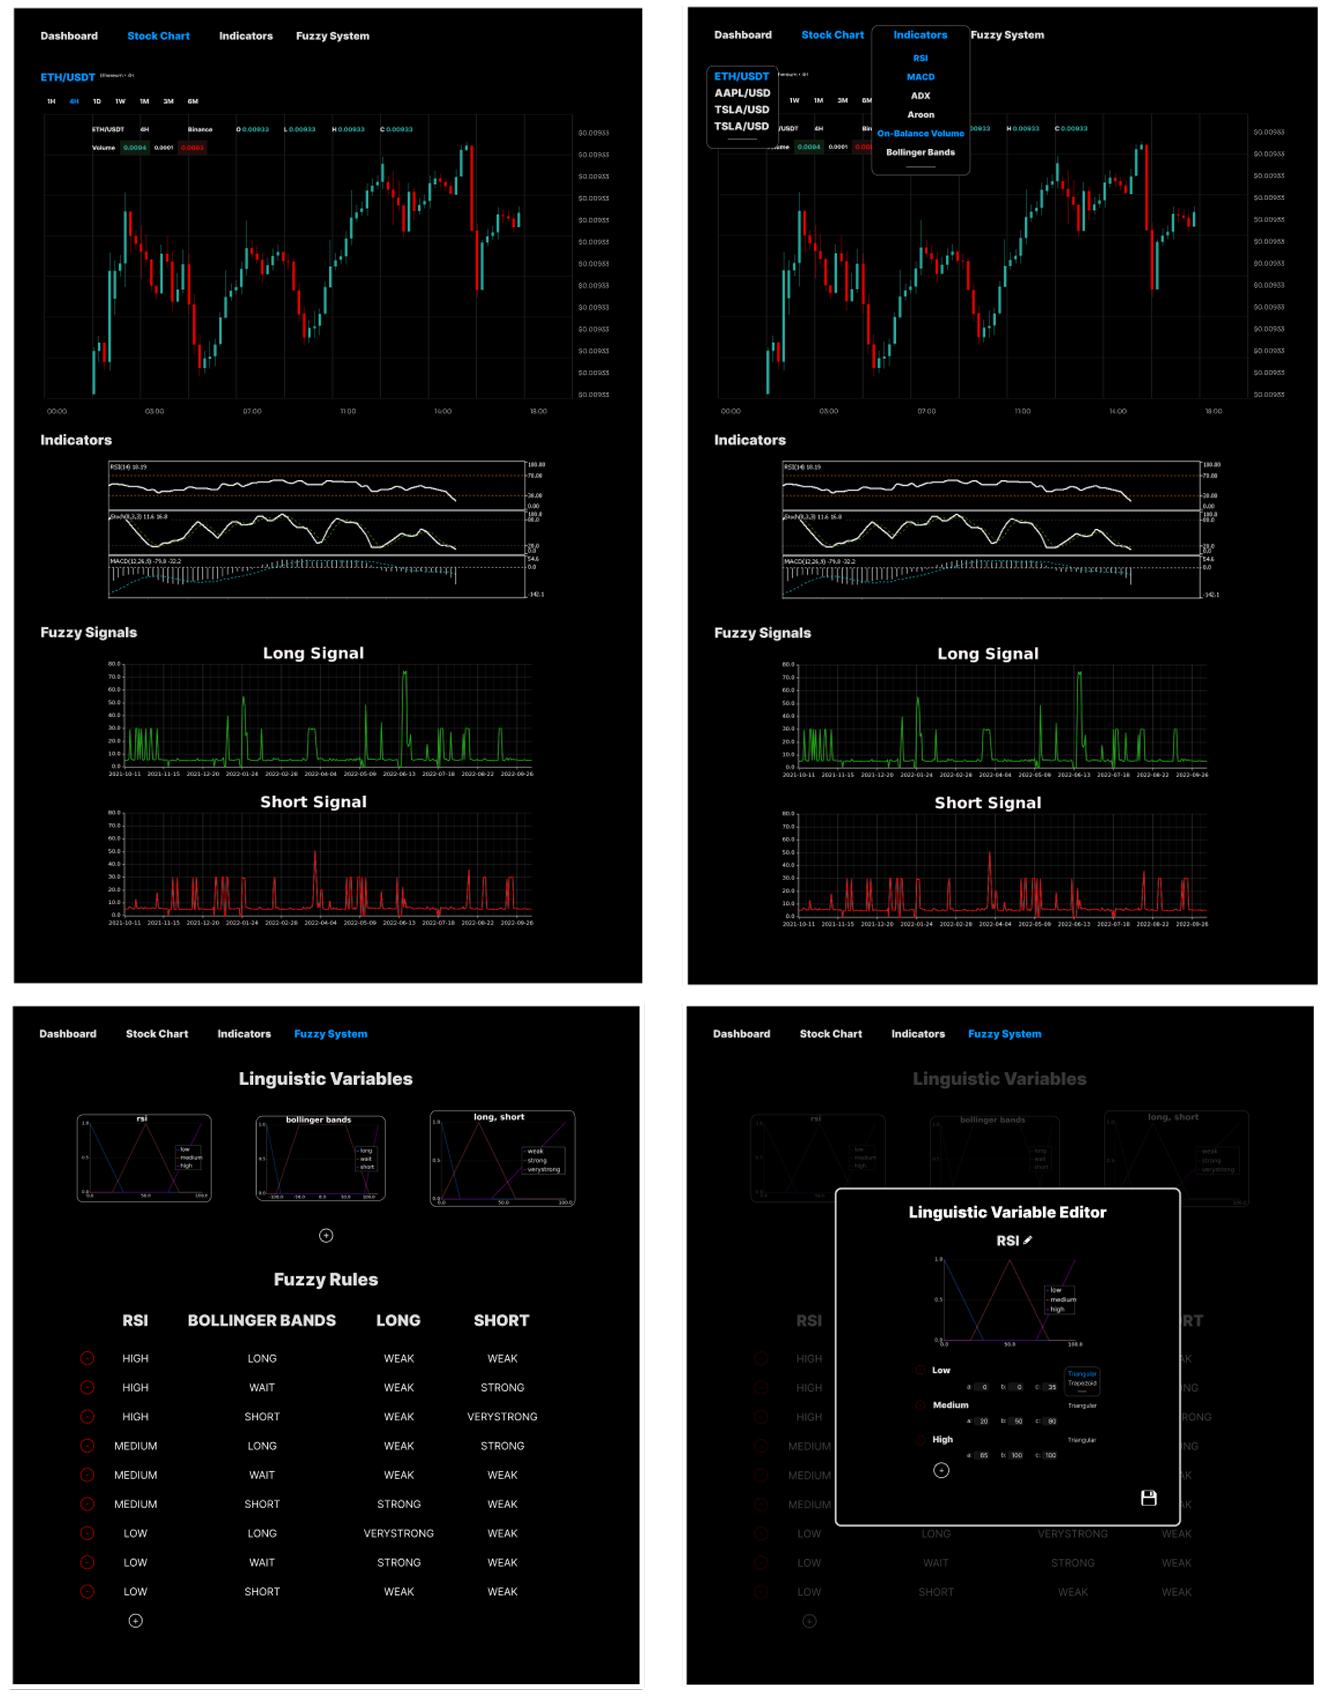
\includegraphics[width=\textwidth]{images/web_uiux.png}
    \caption{UI/UX ของเว็บไซต์}
\end{figure}

%\chapter{\ifenglish Manual\else คู่มือการใช้งานระบบ\fi}
%Manual goes here.

\subsubsection{การตั้งค่าของตัวชี้วัด}
\begin{figure}[ht]
    \centering
    \subfigure[aroon up]{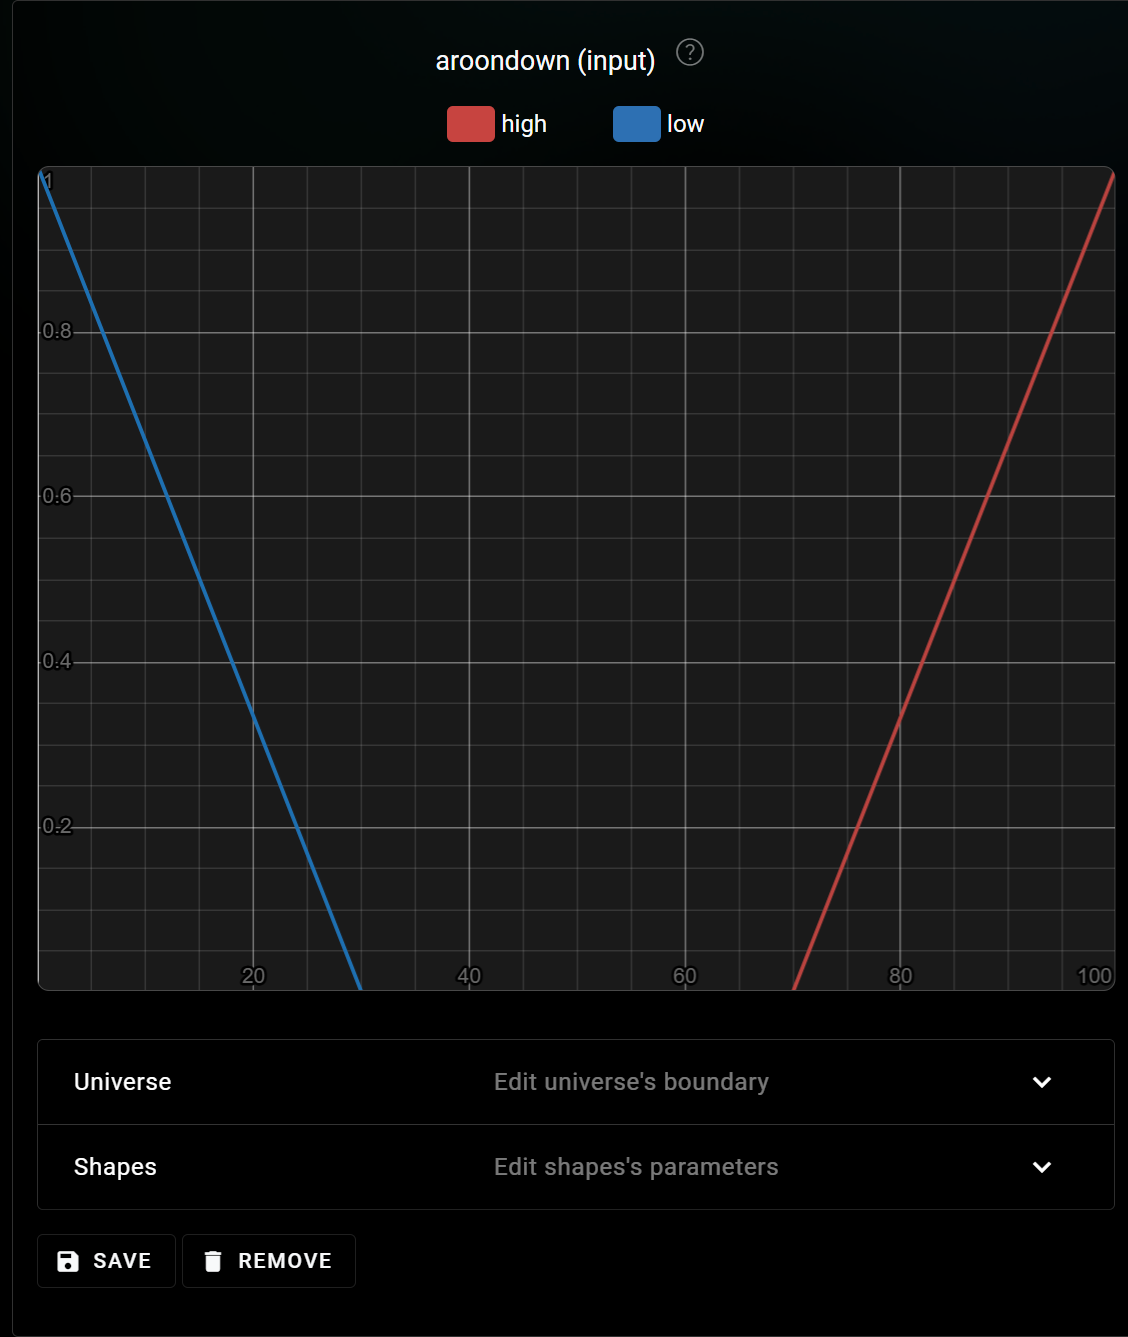
\includegraphics[width=0.4\textwidth]{images/aroon-macd/aroondown.png}}
    \subfigure[aroon down]{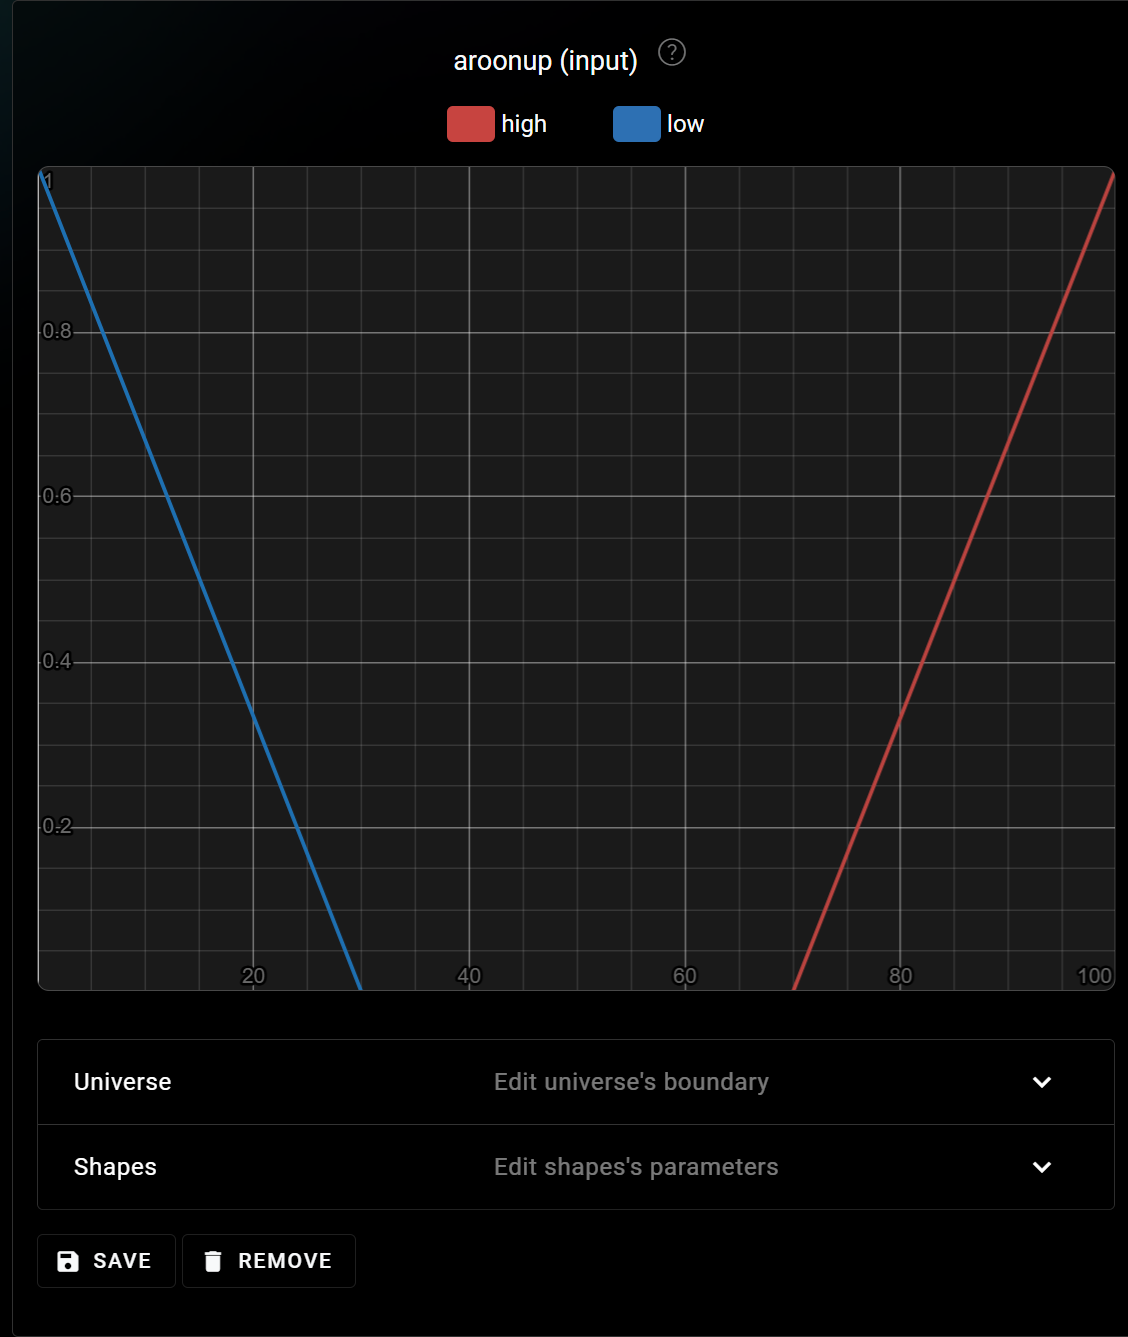
\includegraphics[width=0.4\textwidth]{images/aroon-macd/aroonup.png}}
    \subfigure[macd]{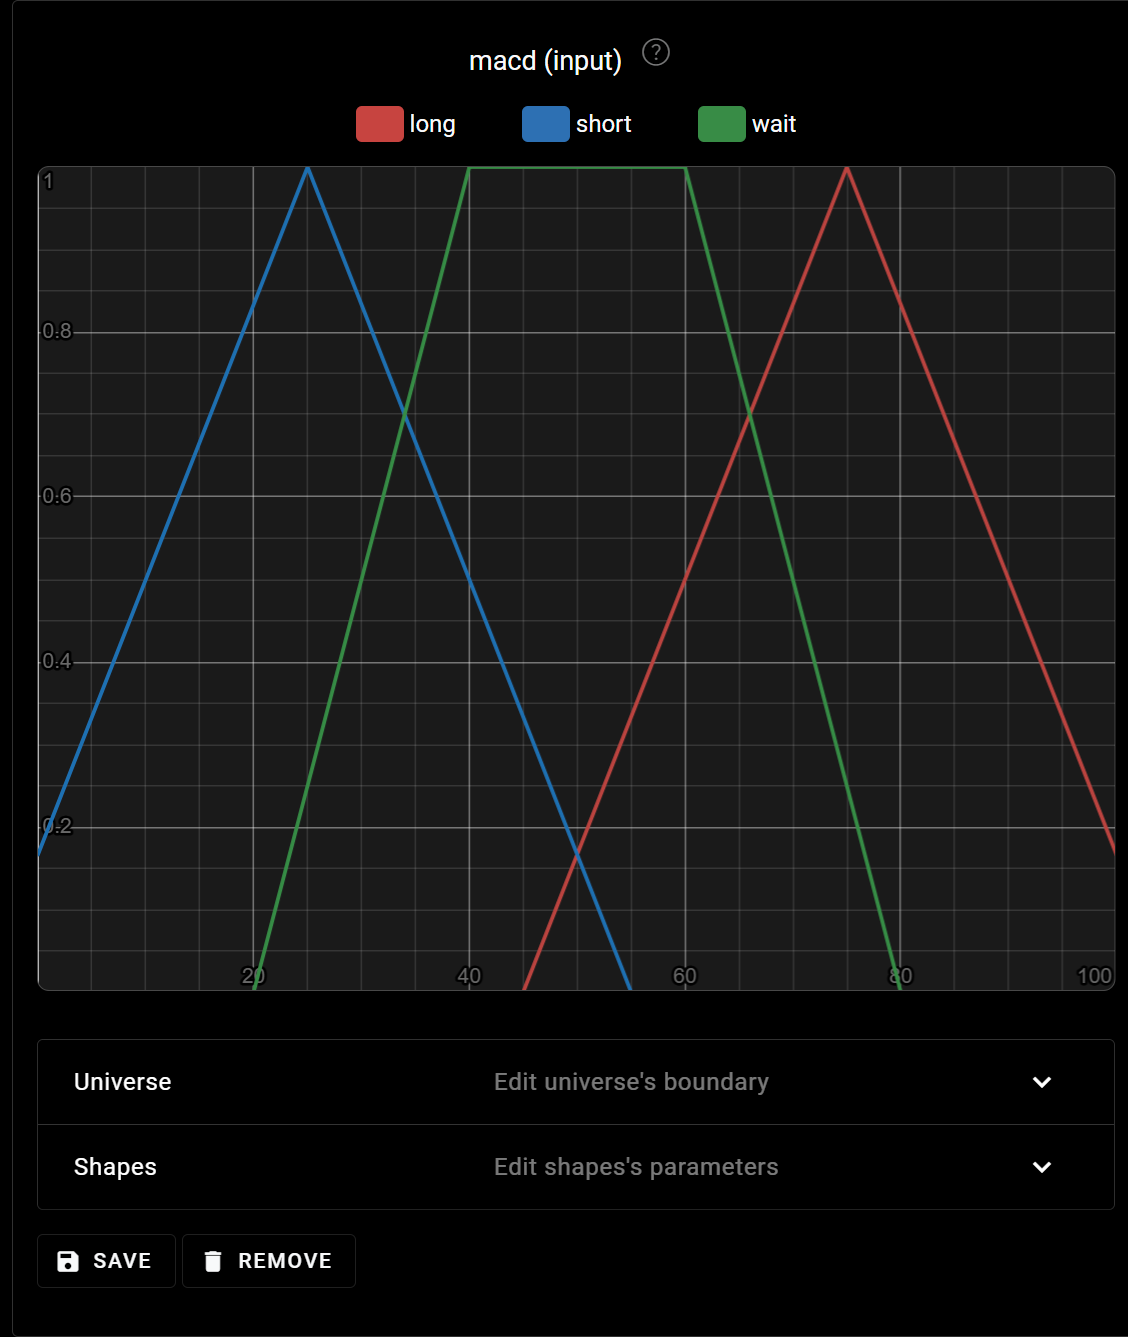
\includegraphics[width=0.4\textwidth]{images/aroon-macd/macd.png}}
    \subfigure[long]{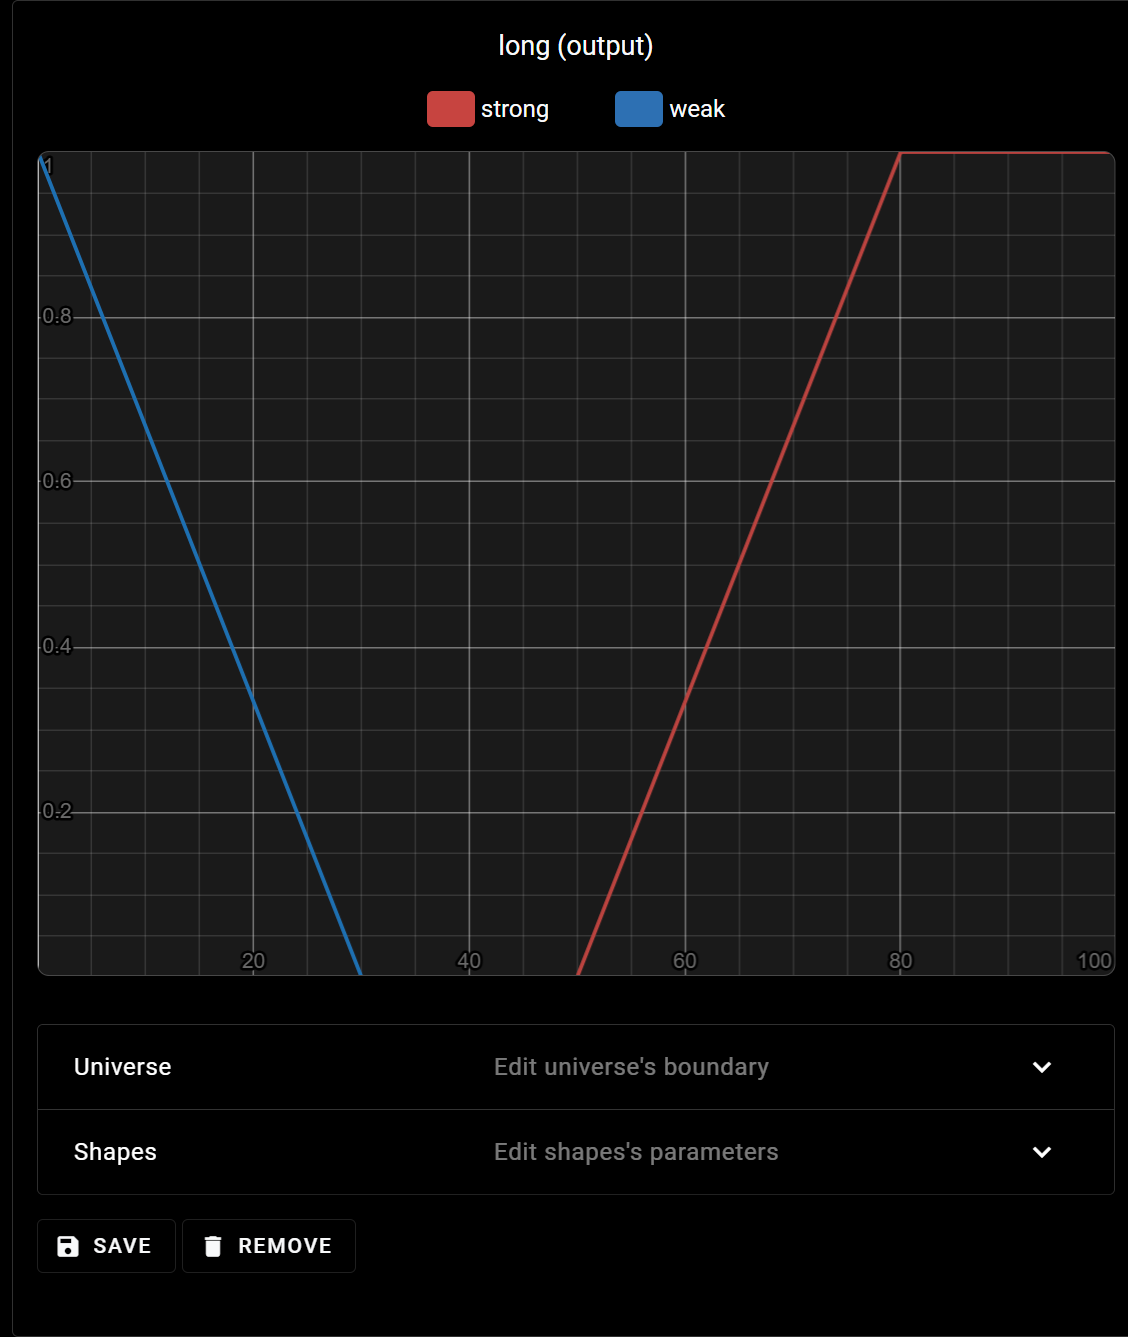
\includegraphics[width=0.4\textwidth]{images/aroon-macd/long.png}}
    \subfigure[short]{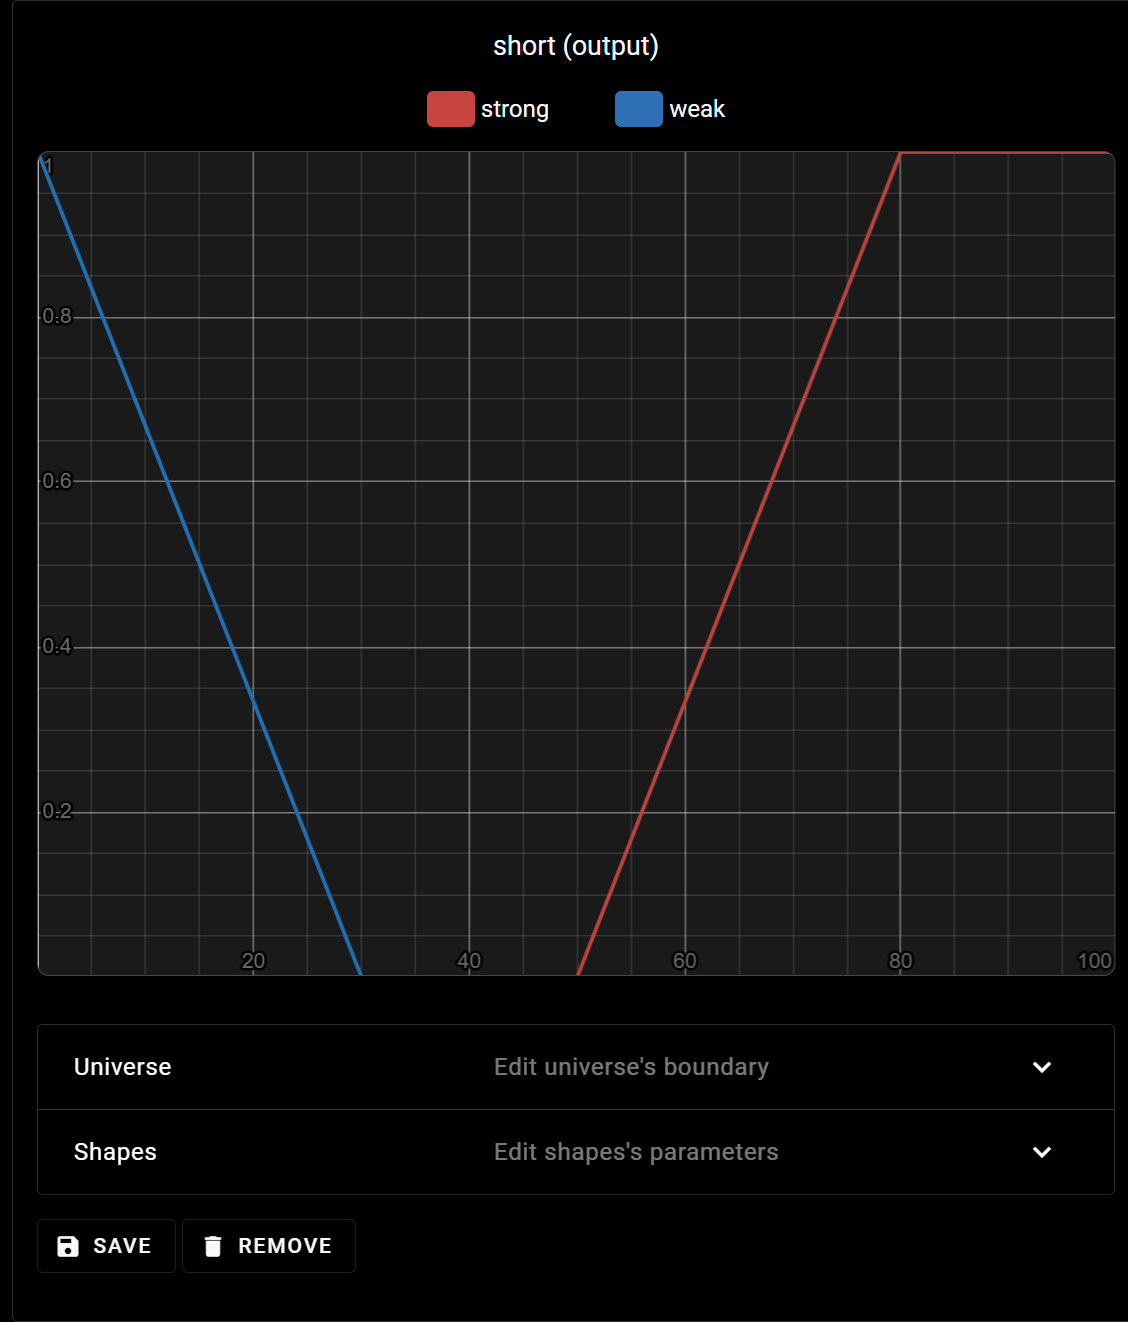
\includegraphics[width=0.4\textwidth]{images/aroon-macd/short.png}}
    \caption{ตัวแปรทางภาษาของตัวชี้วัด AROON-MACD จากในระบบของเรา}
    \label{fig:aroon-macd-lin}
\end{figure}

\begin{figure}[ht]
    \centering
    \subfigure[bollinger band]{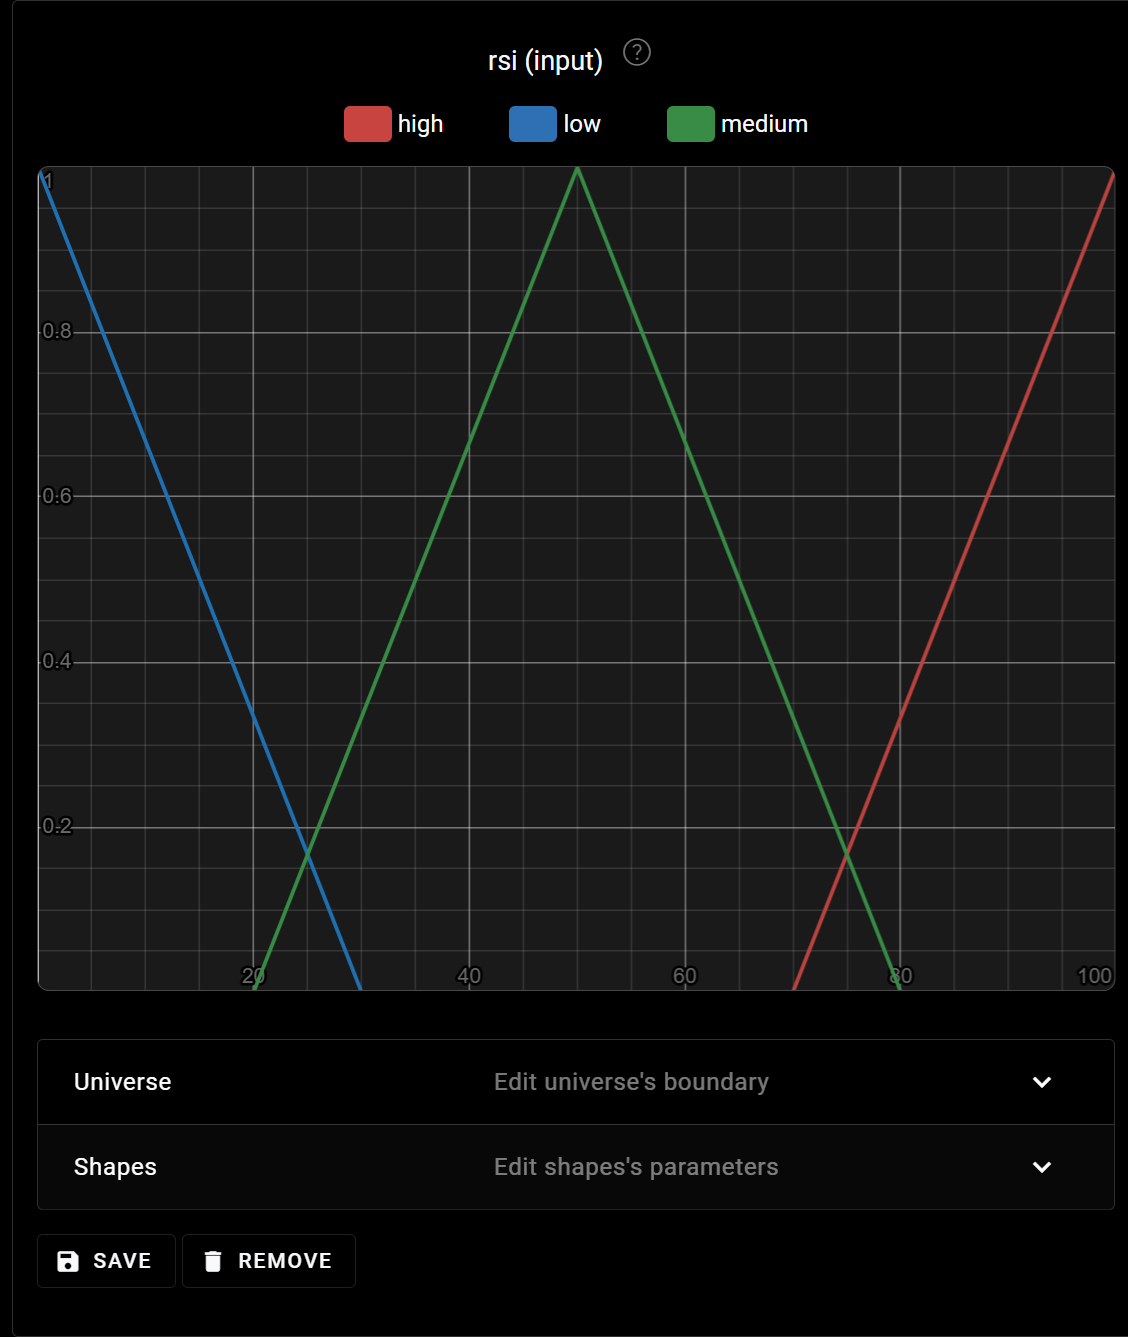
\includegraphics[width=0.4\textwidth]{images/rsi-bb/rsi.png}}
    \subfigure[rsi]{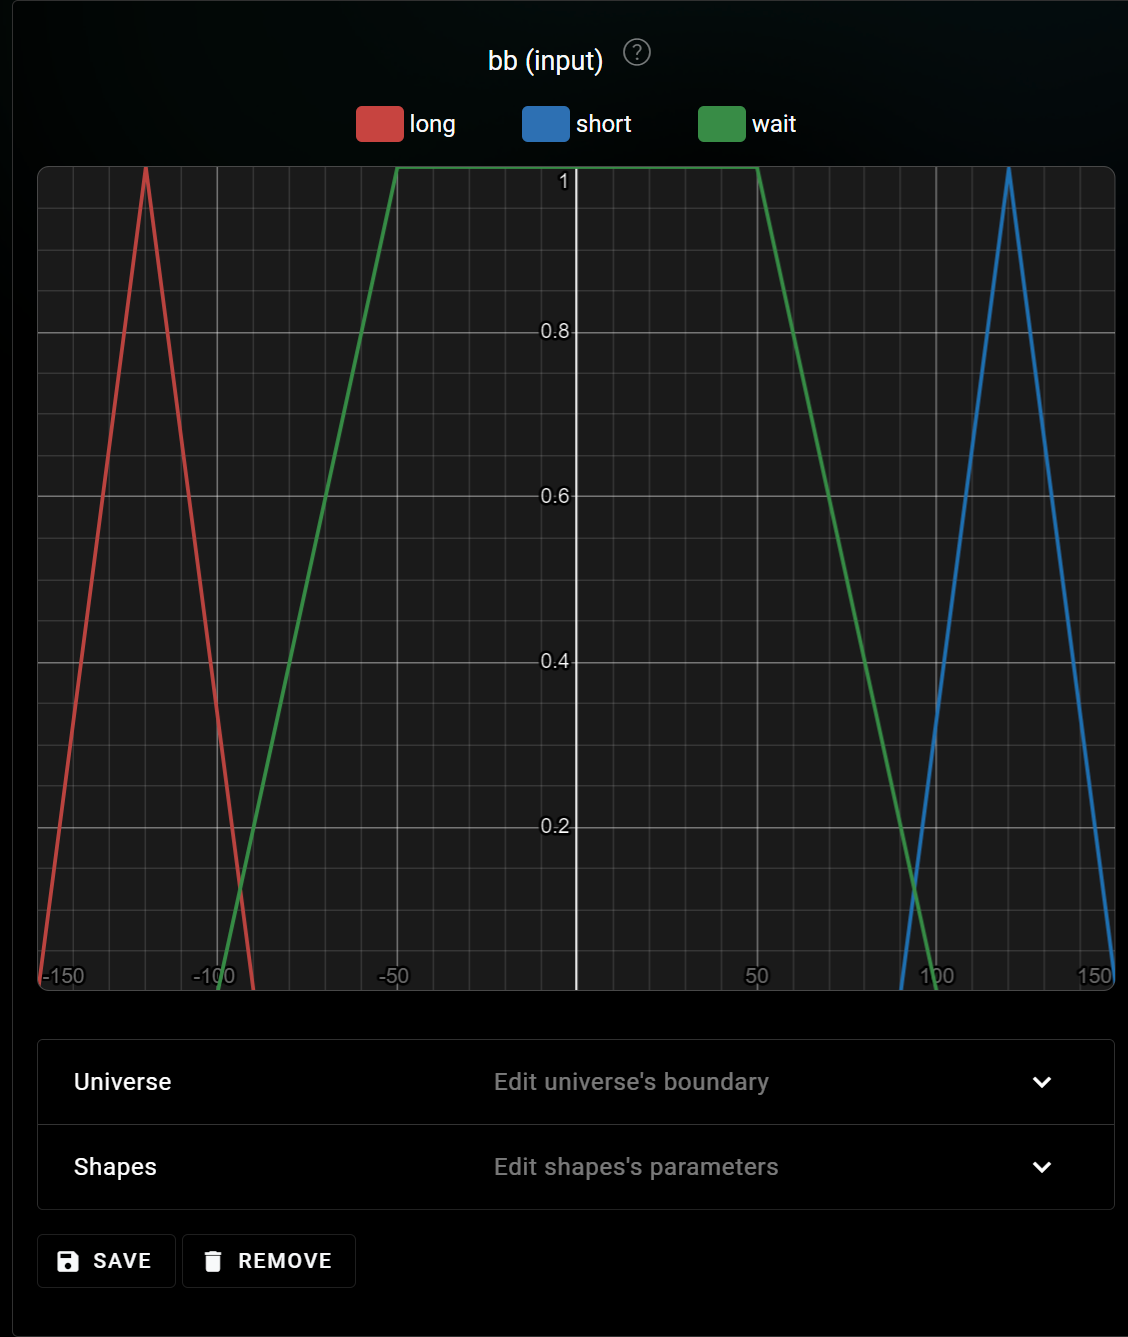
\includegraphics[width=0.4\textwidth]{images/rsi-bb/bb.png}}
    \subfigure[long]{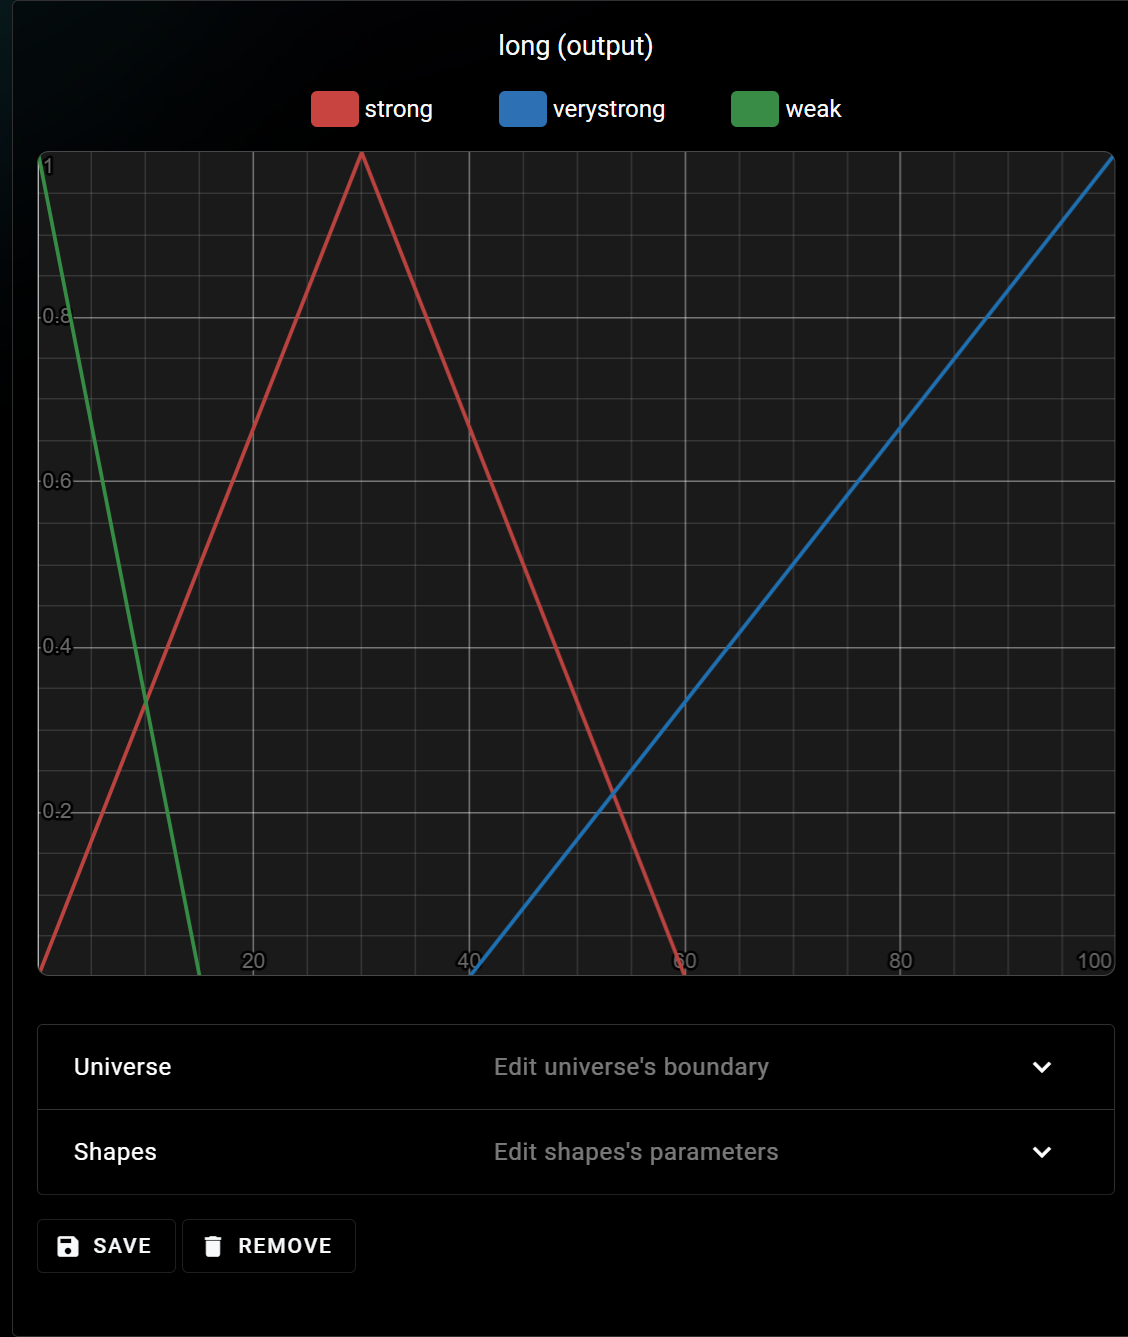
\includegraphics[width=0.4\textwidth]{images/rsi-bb/long.png}}
    \subfigure[short]{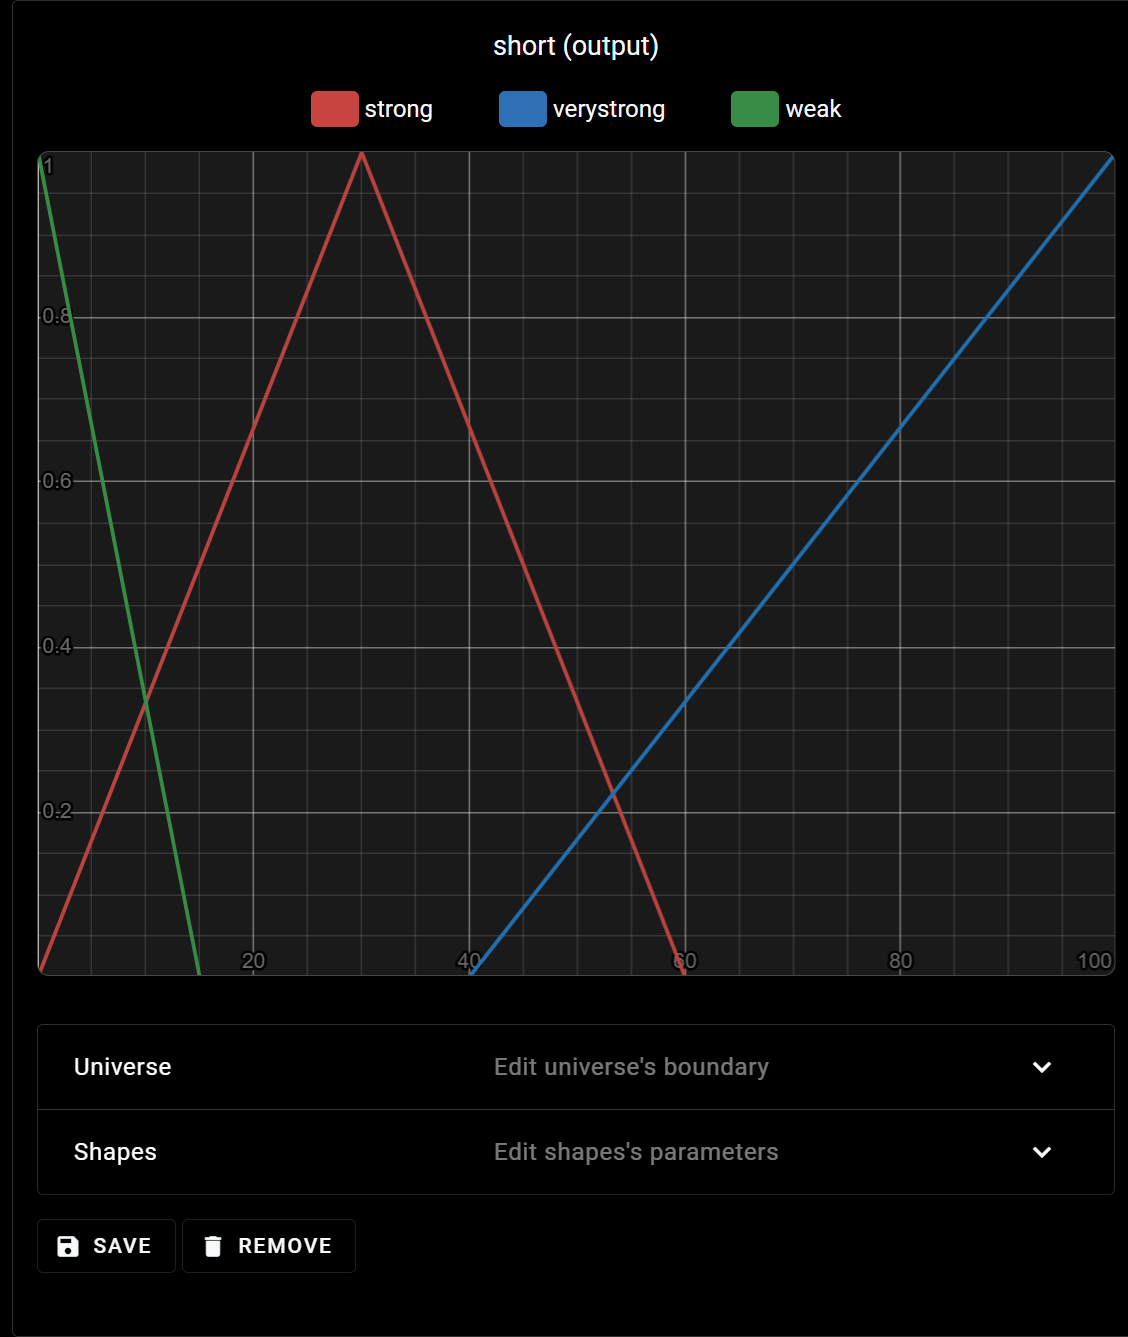
\includegraphics[width=0.4\textwidth]{images/rsi-bb/short.png}}
    \caption{ตัวแปรทางภาษาของตัวชี้วัด RSI-BB จากในระบบของเรา}
    \label{fig:rsi-bb-lin}
\end{figure}

\subsubsection{ผลลัพธ์จากการใช้ PSO ฝึกสอน}
\begin{figure}[ht]
    \centering
    \subfigure[]{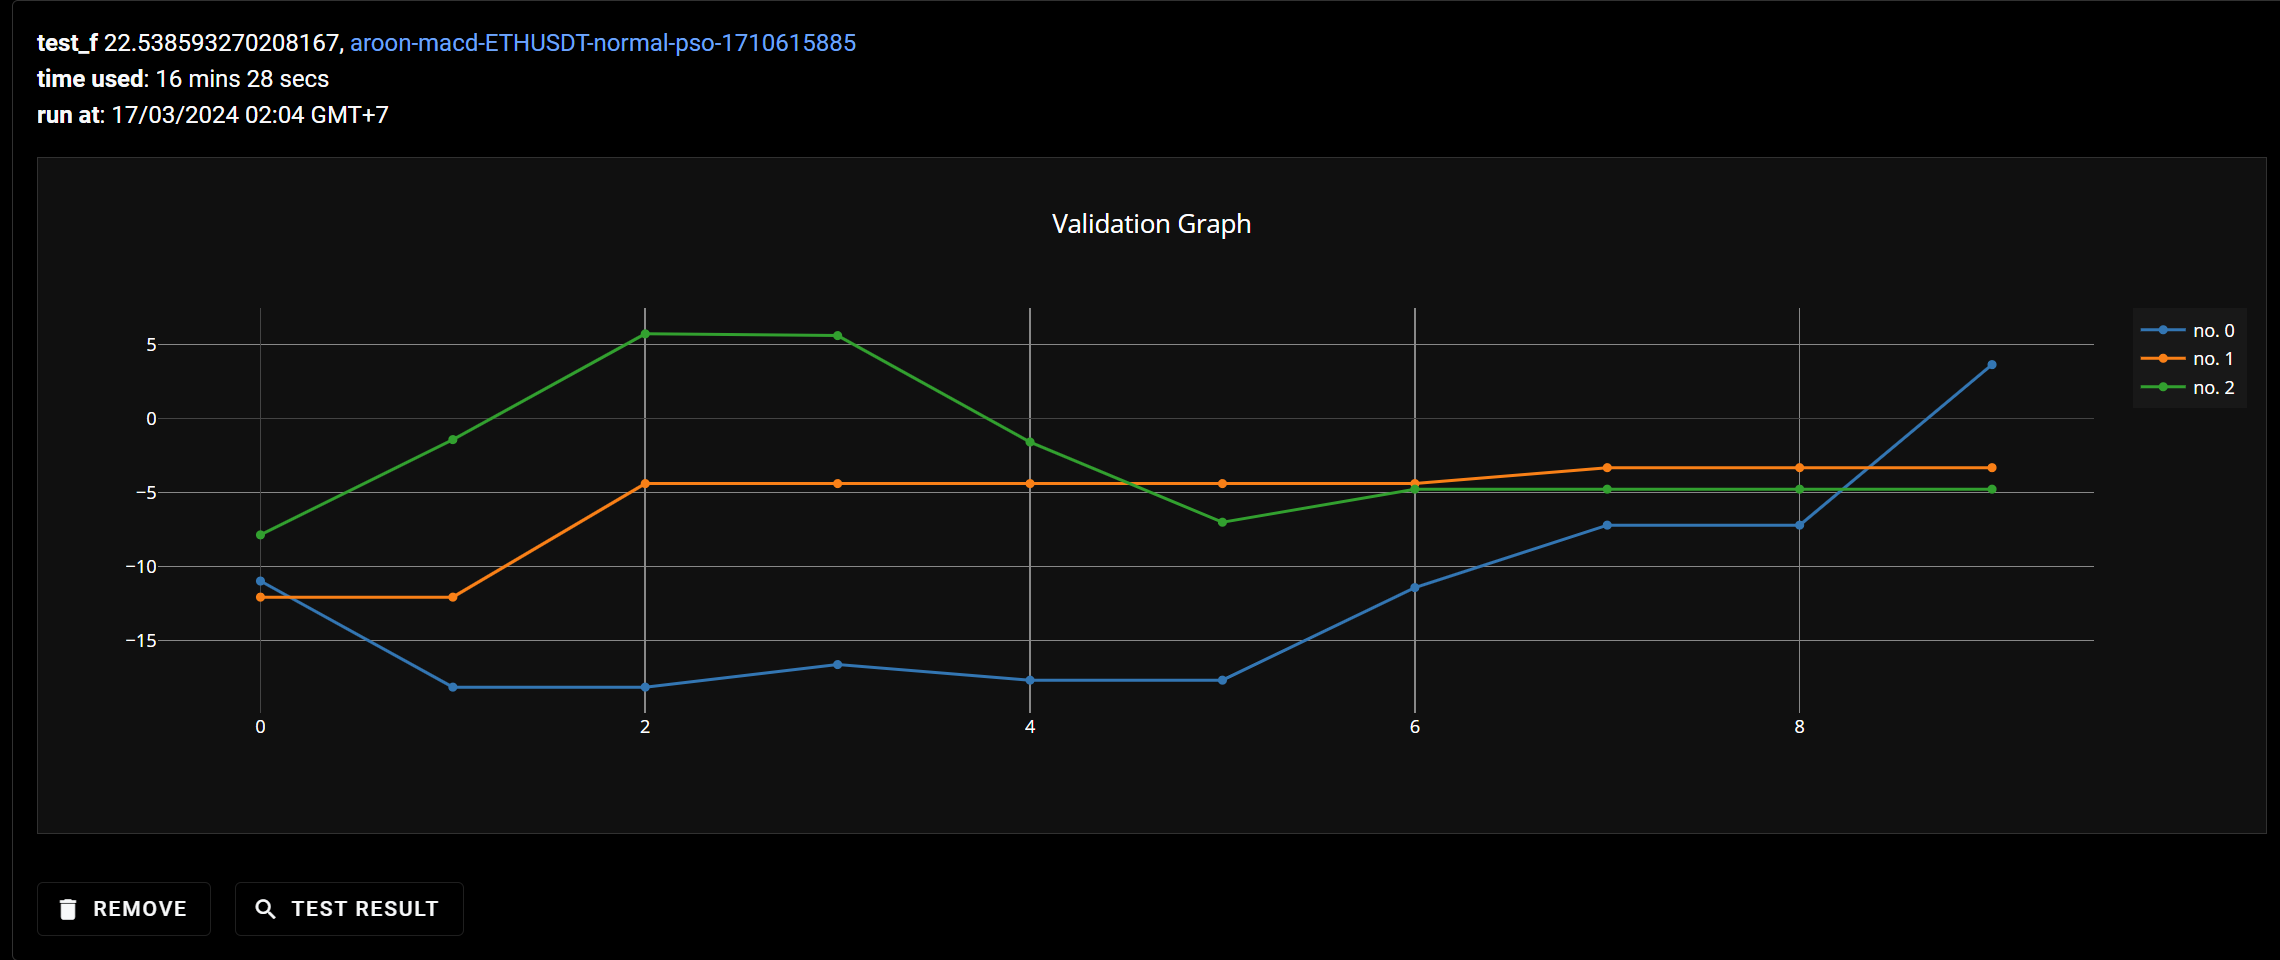
\includegraphics[width=0.5\textwidth]{images/pso/aroon-macd/eth-normal.png}}
    \subfigure[]{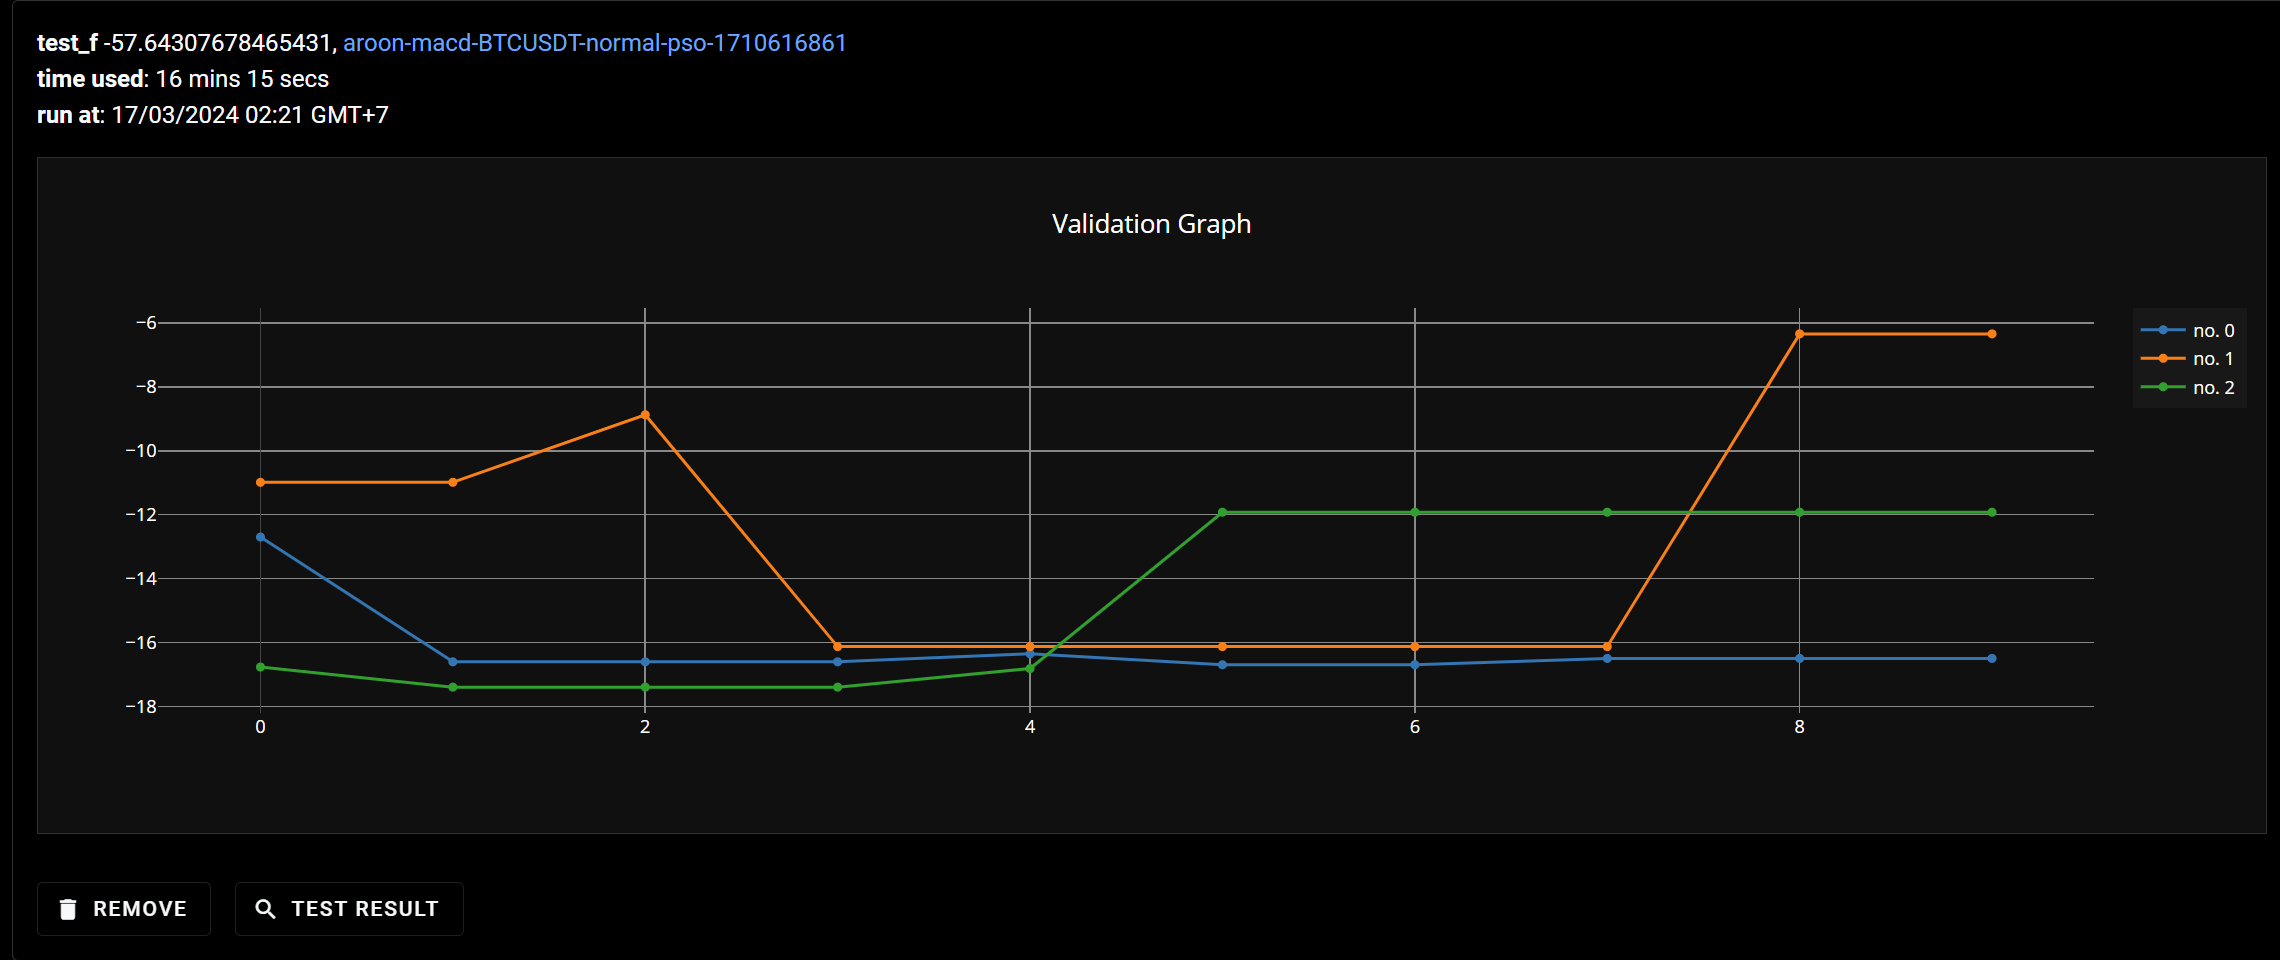
\includegraphics[width=0.5\textwidth]{images/pso/aroon-macd/btc-normal.png}}
    \subfigure[]{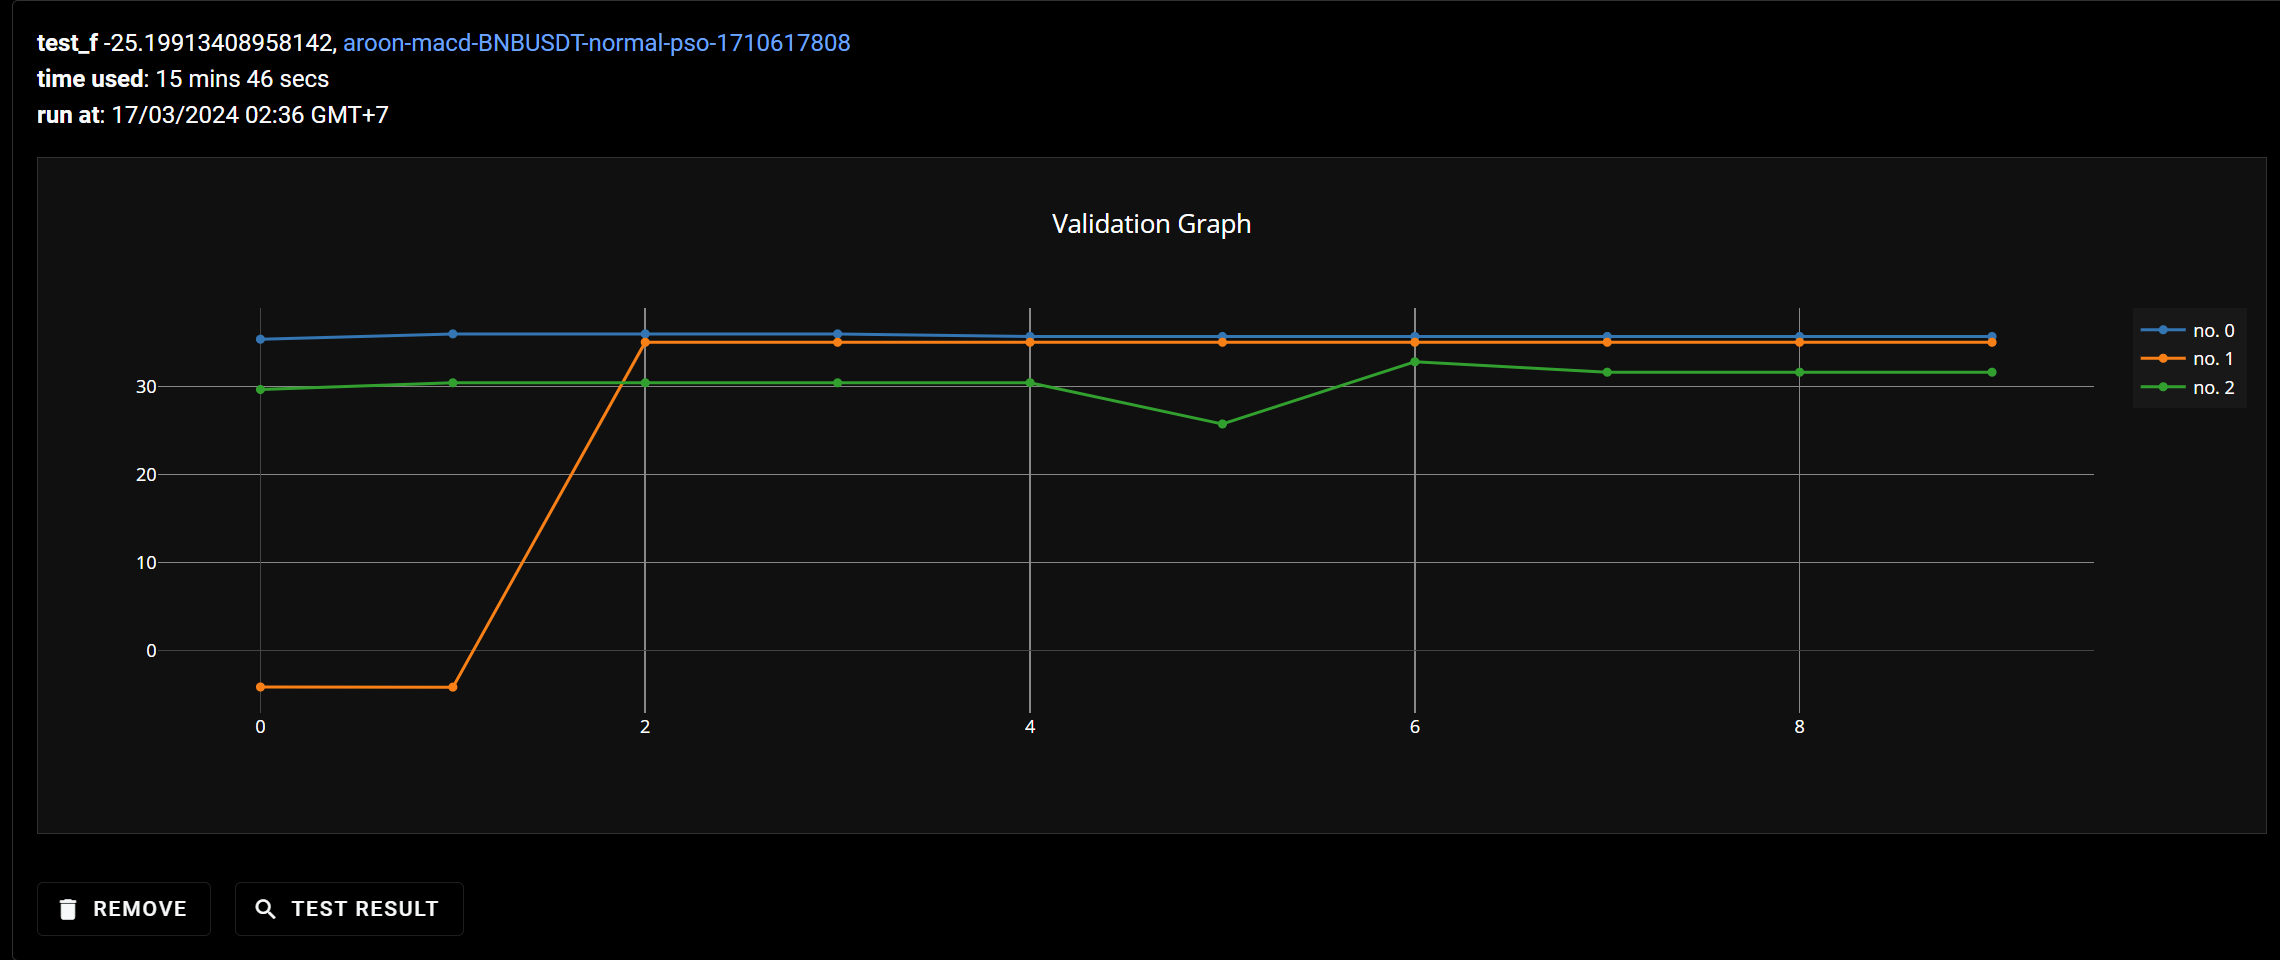
\includegraphics[width=0.5\textwidth]{images/pso/aroon-macd/bnb-normal.png}}
    \subfigure[]{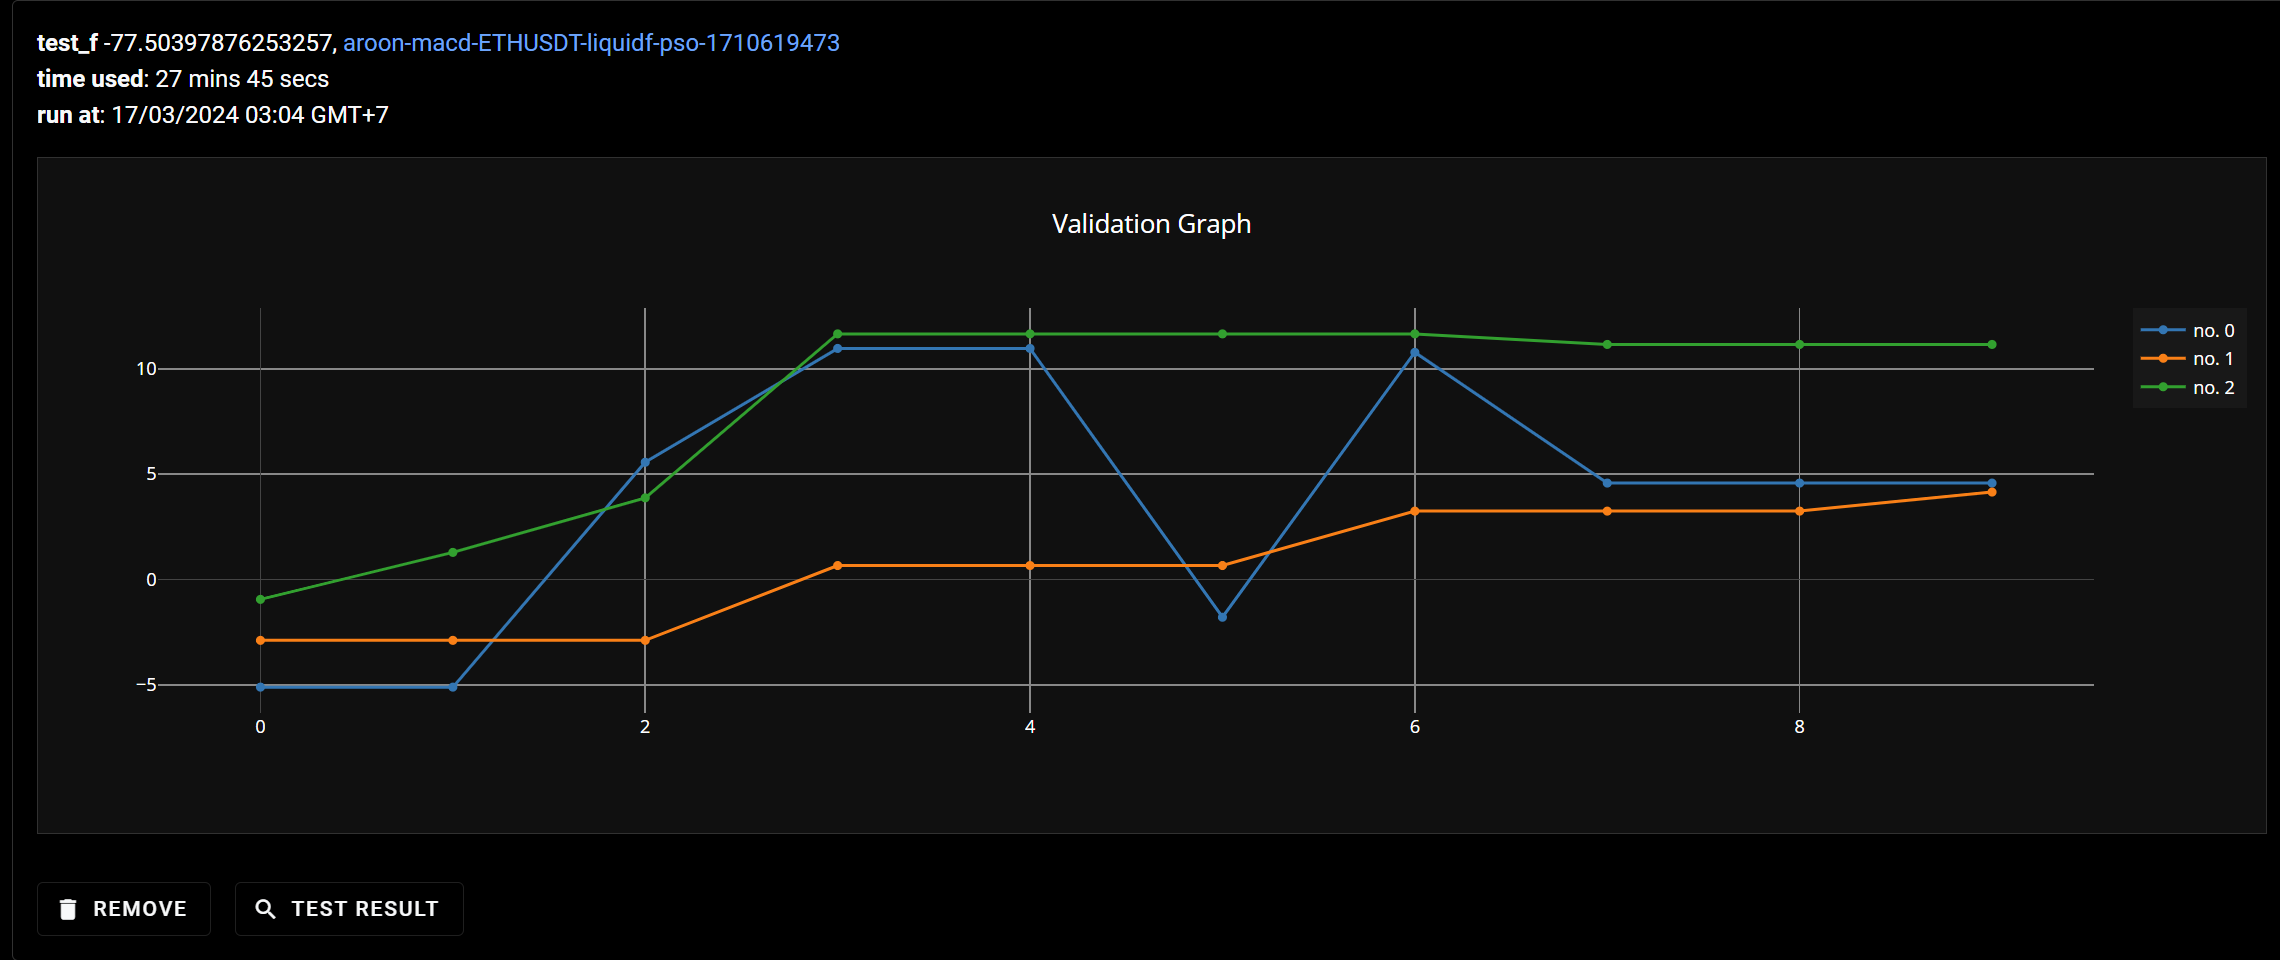
\includegraphics[width=0.5\textwidth]{images/pso/aroon-macd/eth-liquid.png}}
    \subfigure[]{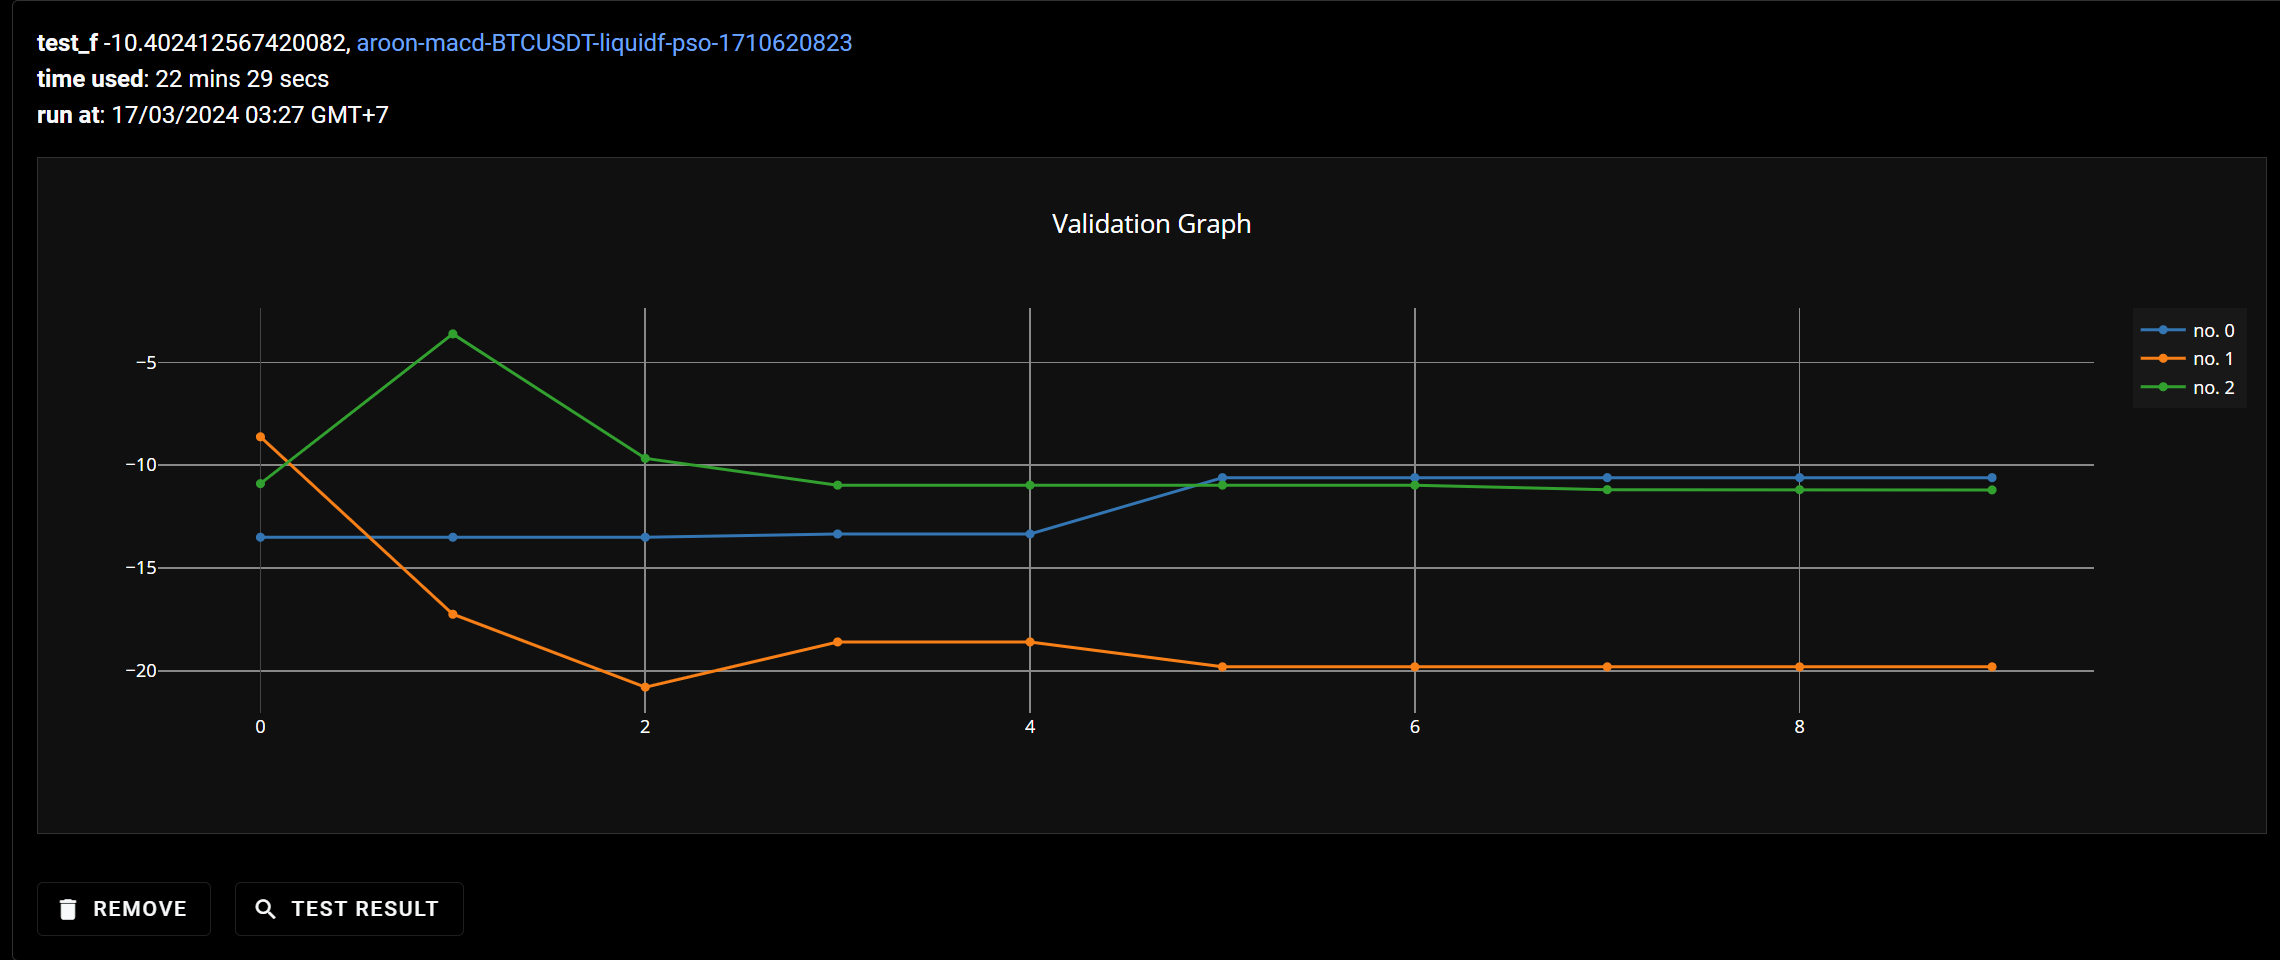
\includegraphics[width=0.5\textwidth]{images/pso/aroon-macd/btc-liquid.png}}
    \subfigure[]{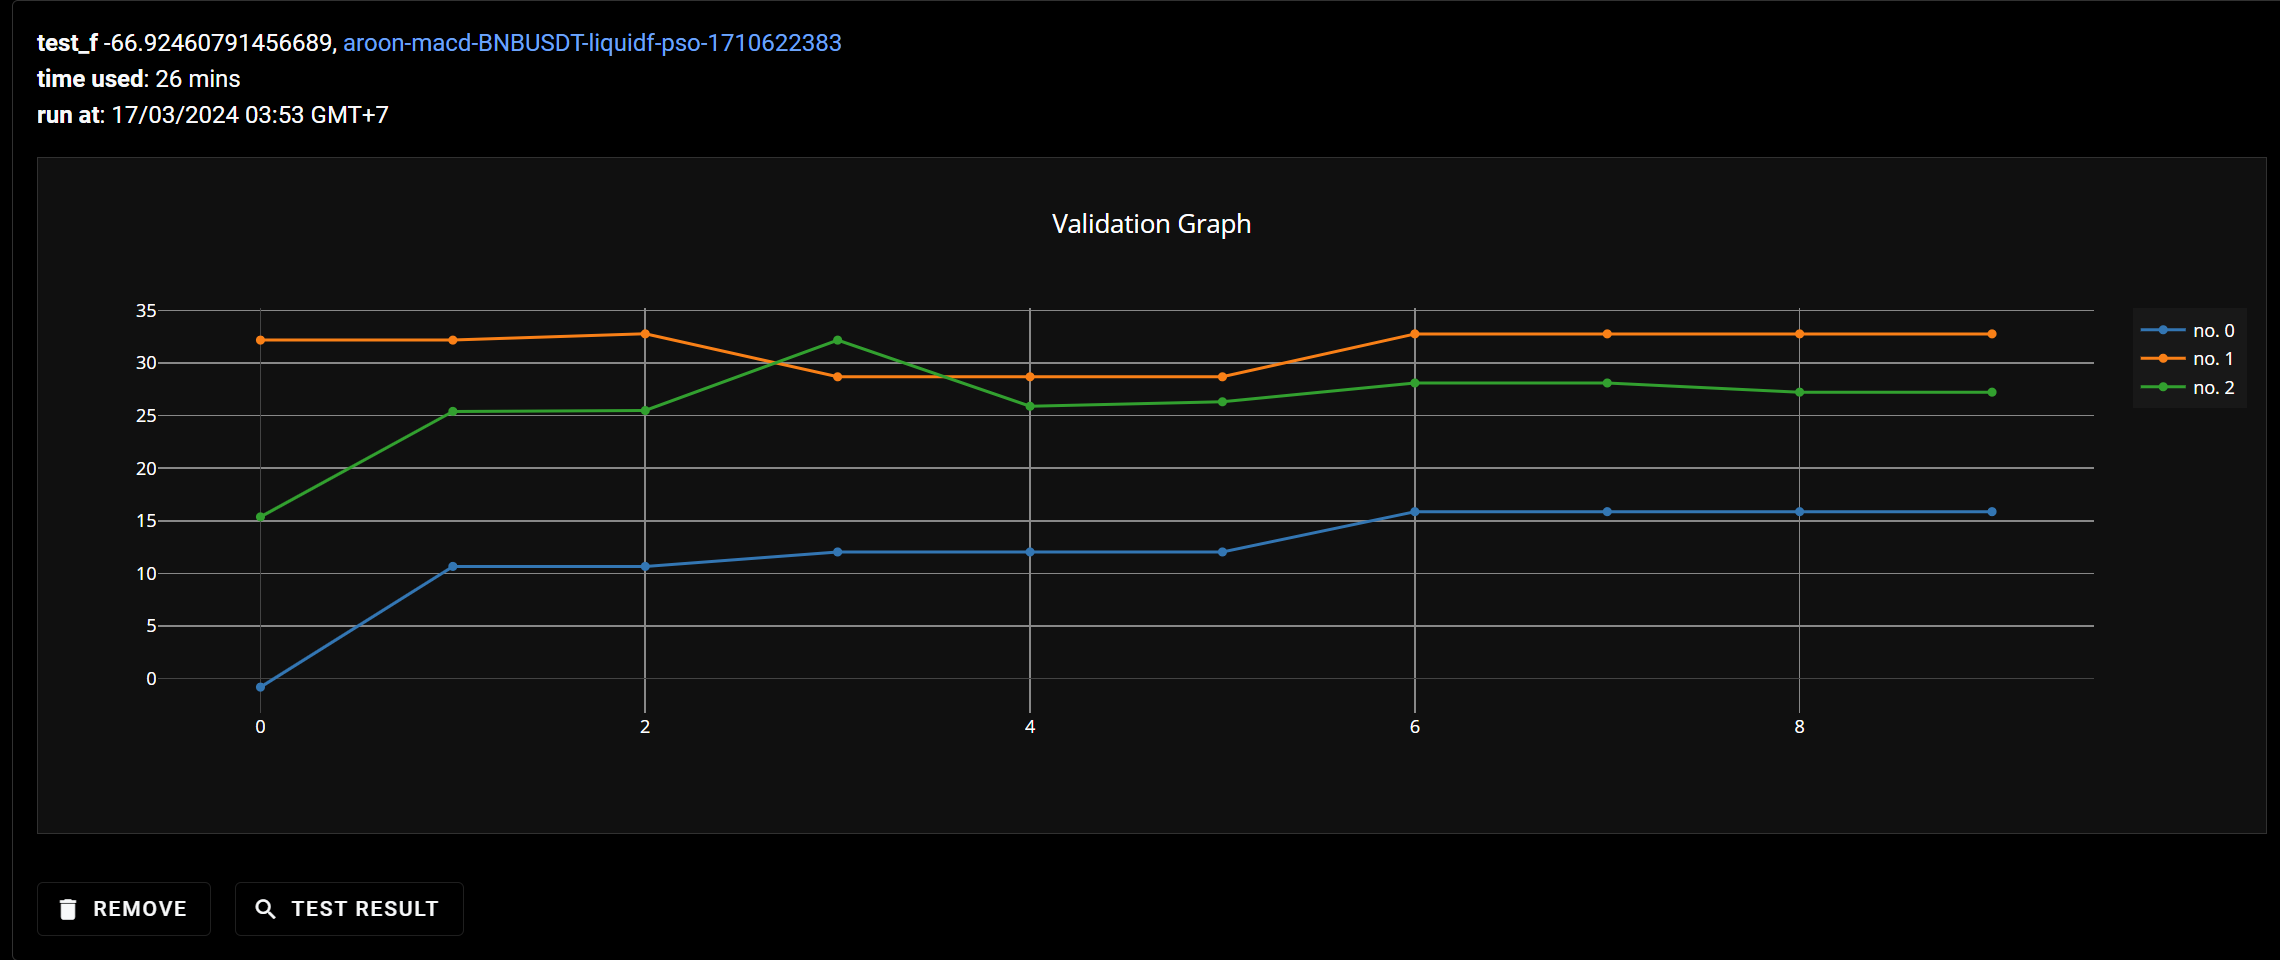
\includegraphics[width=0.5\textwidth]{images/pso/aroon-macd/bnb-liquid.png}}
    \caption{}
\end{figure}